78. \begin{figure}[ht!]
\center{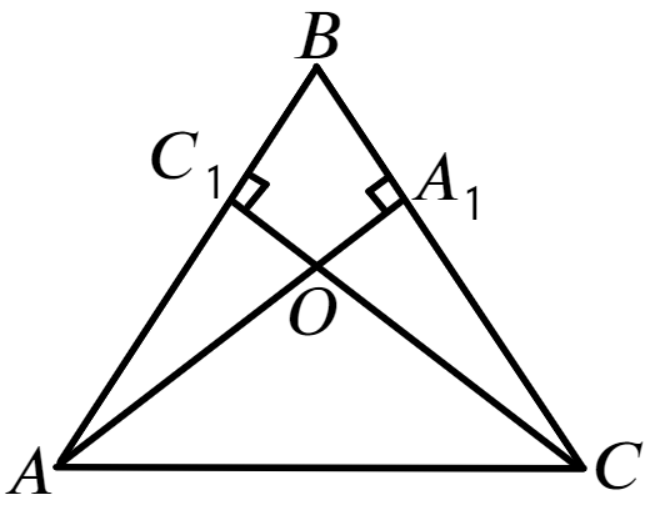
\includegraphics[scale=0.35]{g8-78.png}}
\end{figure}\\
Из четырёхугольника $OC_1BA_1:\ \angle C_1OA_1=360^\circ-90^\circ-90^\circ-70^\circ=110^\circ.$ Так как углом между прямыми по определению считается острый (или прямой) угол, ответом будет $180^\circ-110^\circ=70^\circ.$\newpage\noindent
